\chaptermark{Supplementary Material}
\section*{1. Further parameters for Chapter \ref{chap:VEC}}

This section of the supplementary contains detail on the standardisation of parameter names and meanings, as well as explicitly describing relationships between parameters where they exist. Table \ref{table:param} shows standard parameter names for vector models, aligned with Smith et al 2012 \cite{Smith2012}. Table \ref{table:param2} describes additional parameters defined for the purposes of the model used in Chapter \ref{chap:VEC}.

\begin{table*}[h]
\caption{Standard parameter names for vector models (Smith et al 2012).}% title of Table
\vspace{.1cm}
\centering % used for centering table
\begin{tabular}{l c c}% centered columns (4 columns)
\hline\hline                        %inserts double horizontal lines
Definition & Parameter & Notes \\ [0.5ex]% inserts table 
%heading
\hline                  % inserts single horizontal line
Population density of humans & $H$ &  \\
Population density of mosquitoes & $M$ &  \\
Number of infected humans & $X$ &  \\
Number of exposed vectors & $Y$ & $N_E$ \\
Number of infectious vectors & $Z$ & $N_I$ \\
Human blood feeding rate (daily) & $a$ & \\
Probability vector survives one day & $p$ & \\
Instantaneous vector death rate & $g$ & $g=-\ln(p)$  \\
Intrinsic incubation period (in humans) & $u$ & \\
Extrinsic incubation period (in vectors) & $v$ & \\
Human recovery rate & $r$ & \\
Prob vector infected after biting infected human & $c$ & \\
Prob infectious bite infects a human & $b$ & \\
Blood feeding rate (all prey) & $f$ & \\
Fraction of blood meals on humans & $Q$ & $a=fQ$ \\
Mean feeding cycle length & $\delta$ & $a=Q/\delta$\\
Prevalence of malaria in humans & $x$ & \\
Fraction of exposed vectors & $y$ & \\
Fraction of infectious vectors & $z$ & \\
Ratio of vectors to humans & $m$ & $=M/H$ \\
Human biting rate (\# bites per human per day) & $HBR$ & $=ma$\\
EIR (\# infectious bites per human per day) & $E$ & $=maz$ \\
The average mosquito lifespan & $1/g$ & \\
Stability index (\# human bites per vector across its life) & $S$ & $=a/g$\\
Probability vector survives to infectiousness & $P$ & $=e^{-gv}$\\
Probability vector infected during human bloodmeal & $\kappa$ & $=cx$\\
Vectorial capacity & $V$ & \\
Basic reproductive number & $R_0$ & \\
Effective reproductive number under control & $R_c$ & \\
Critical vector density required to sustain transmission & $m'$ & \\
      % [1ex] adds vertical space
\hline%inserts single line
\end{tabular}
\label{table:param}% is used to refer this table in the text
\end{table*}

\begin{table*}[h!]
\caption{Additional parameter names required for this model.}% title of Table
\vspace{.1cm}
\centering % used for centering table
\begin{tabular}{l c c}% centered columns (4 columns)
\hline\hline                        %inserts double horizontal lines
Definition & Parameter & Notes \\ [0.5ex]% inserts table 
%heading
\hline                  % inserts single horizontal line
Rate of moving from Exposed to Fed & $\pi_2$ & \\
Rate of moving from Fed to Resting & $\pi_3$ & \\
Rate of moving from Resting to Ovipositing & $\pi_4$ & \\
Rate of moving from Ovipositing to Exposed & $\pi_1$ & \\
Emergence rate (from larval stages) & $\beta$ & \\
Linear reduction in emergence rate due to larvicides & $\theta$ & \\
Additional IRS-induced death rate & $\gamma$ & \\
Bednet coverage & $\omega$ & \\
Probability successful feed in presence of bednet & $\sigma$ & \\
Probability death caused by bednet & $\nu$ & \\
Probability successful feed on single attempt & $q_1$ & $=1-Q\omega(1-\sigma)$ \\
Probability death on a single feeding attempt & $q_2$ & $=Q\omega\nu$\\
Probability a vector survives one feeding cycle & $K$ & previously $C$\\
The number of newly emerged null-parous vectors & $B_0$ &\\
Extrinsic incubation period (number of feeding cycles) & $N$ & \\
Probability of vector infection from one bite & $\hat{p}$ & $=xc$ \\
\hline%inserts single line
\end{tabular}
\label{table:param2}% is used to refer this table in the text
\end{table*}

\FloatBarrier

\section*{2. Published article 1}

\textbf{Title:} Seasonally timed treatment programs for Ascaris lumbricoides to increase impact -- An investigation using mathematical models.

\textbf{Authors:} \textbf{Emma L Davis}, Leon Danon, Joaquin M Prada, Sharmini A Gunawardena, James E Truscott, Johnny Vlaminck, Roy M Anderson, Bruno Levecke, Eric R Morgan, T Deirdre Hollingsworth.

\textbf{Journal:} PLOS Neglected Tropical Diseases.

\textbf{Date:} January 2019

\includepdf[pages=-,pagecommand={},width=\textwidth+2cm,offset=20 -20]{STHpaper.pdf}

\section*{3. Published article 2}

\textbf{Title:} Evaluating the evidence for lymphatic filariasis elimination.

\textbf{Authors:} \textbf{Emma L Davis}, Lisa J Reimer, Lorenzo Pellis, T Deirdre Hollingsworth.

\textbf{Journal:} Trends in Parasitology.

\textbf{Date:} November 2019

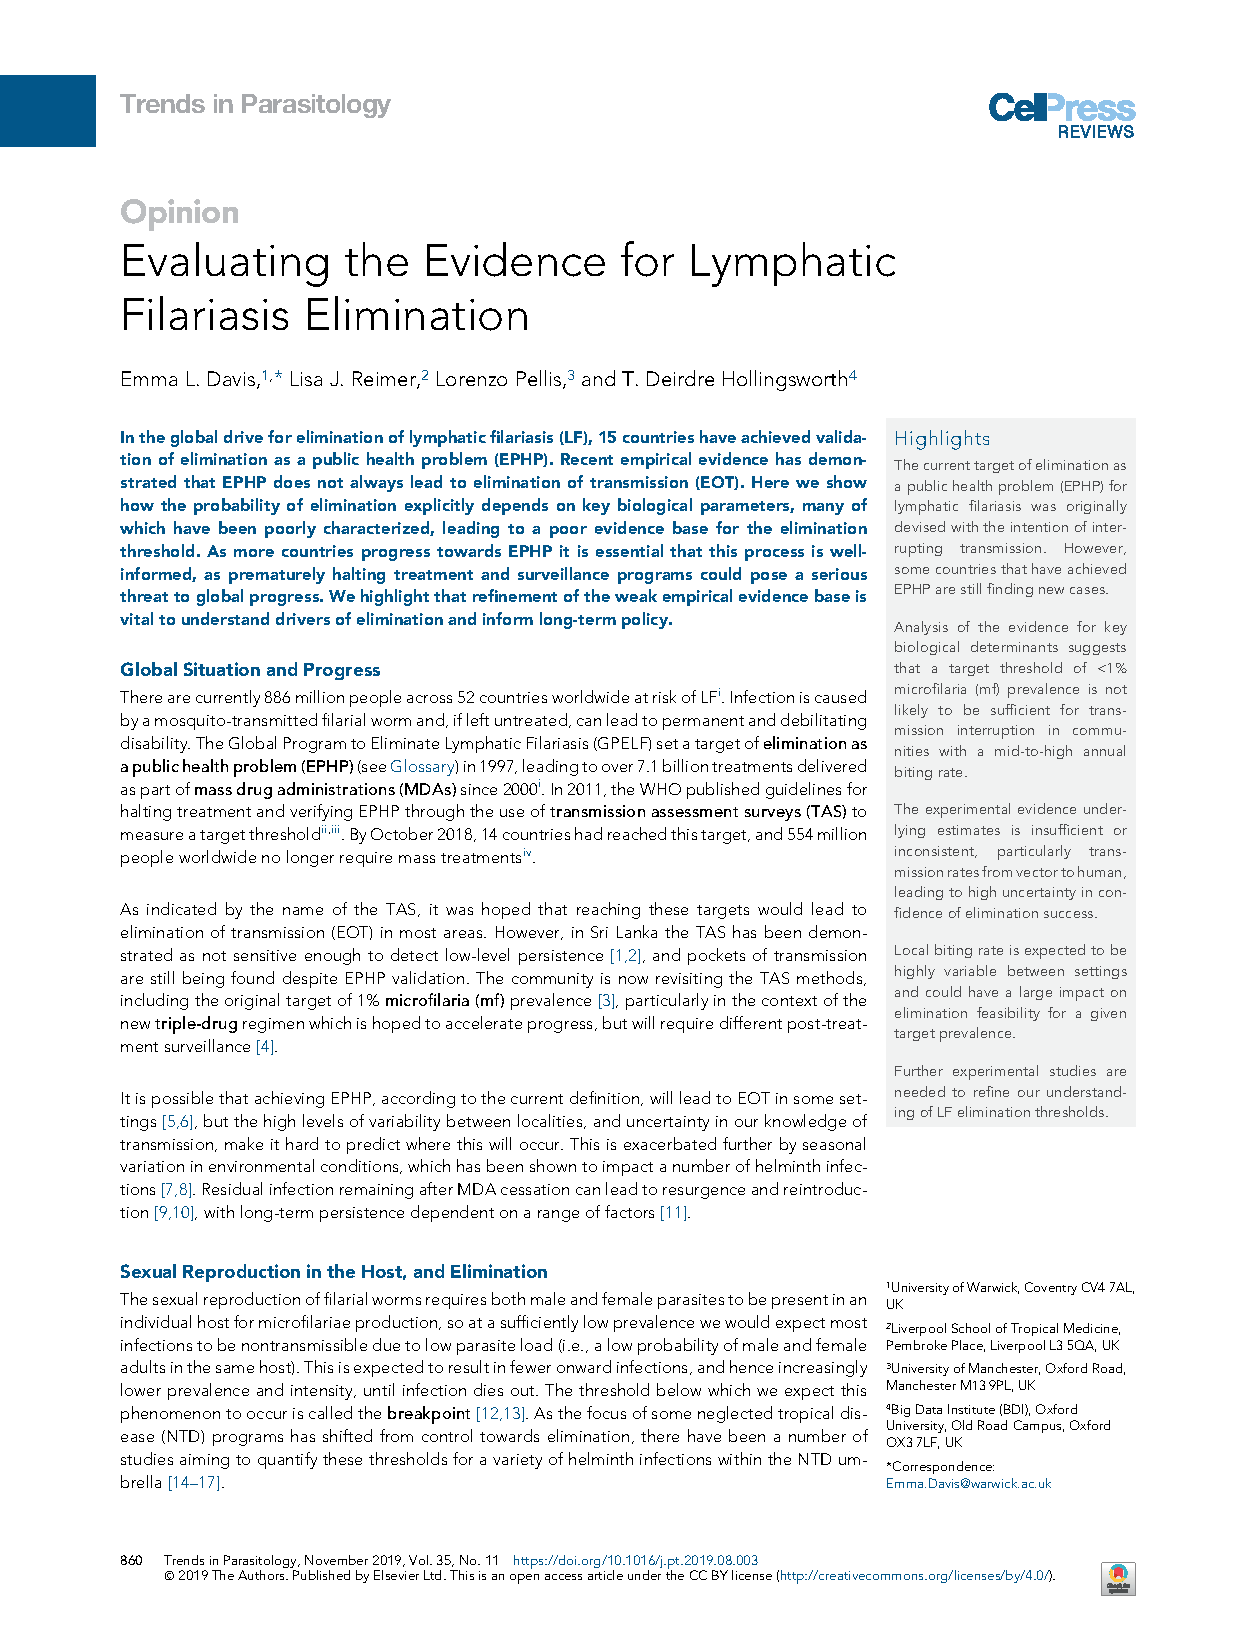
\includepdf[pages=-,pagecommand={},width=\textwidth+2cm,offset=20 -20]{LFpaper.pdf}

\section*{3. Published article 3}

\textbf{Title:} Complex interaction in soil-transmitted helminth co-infections from a cross sectional study in Sri Lanka.

\textbf{Authors:} Hannah C Lepper, Joaquin M Prada, \textbf{Emma L Davis}, Sharmini A Gunawardena, T Deirdre Hollingsworth.

\textbf{Journal:} Transactions of the Royal Society of Tropical Medicine and Hygiene.

\textbf{Date:} June 2018

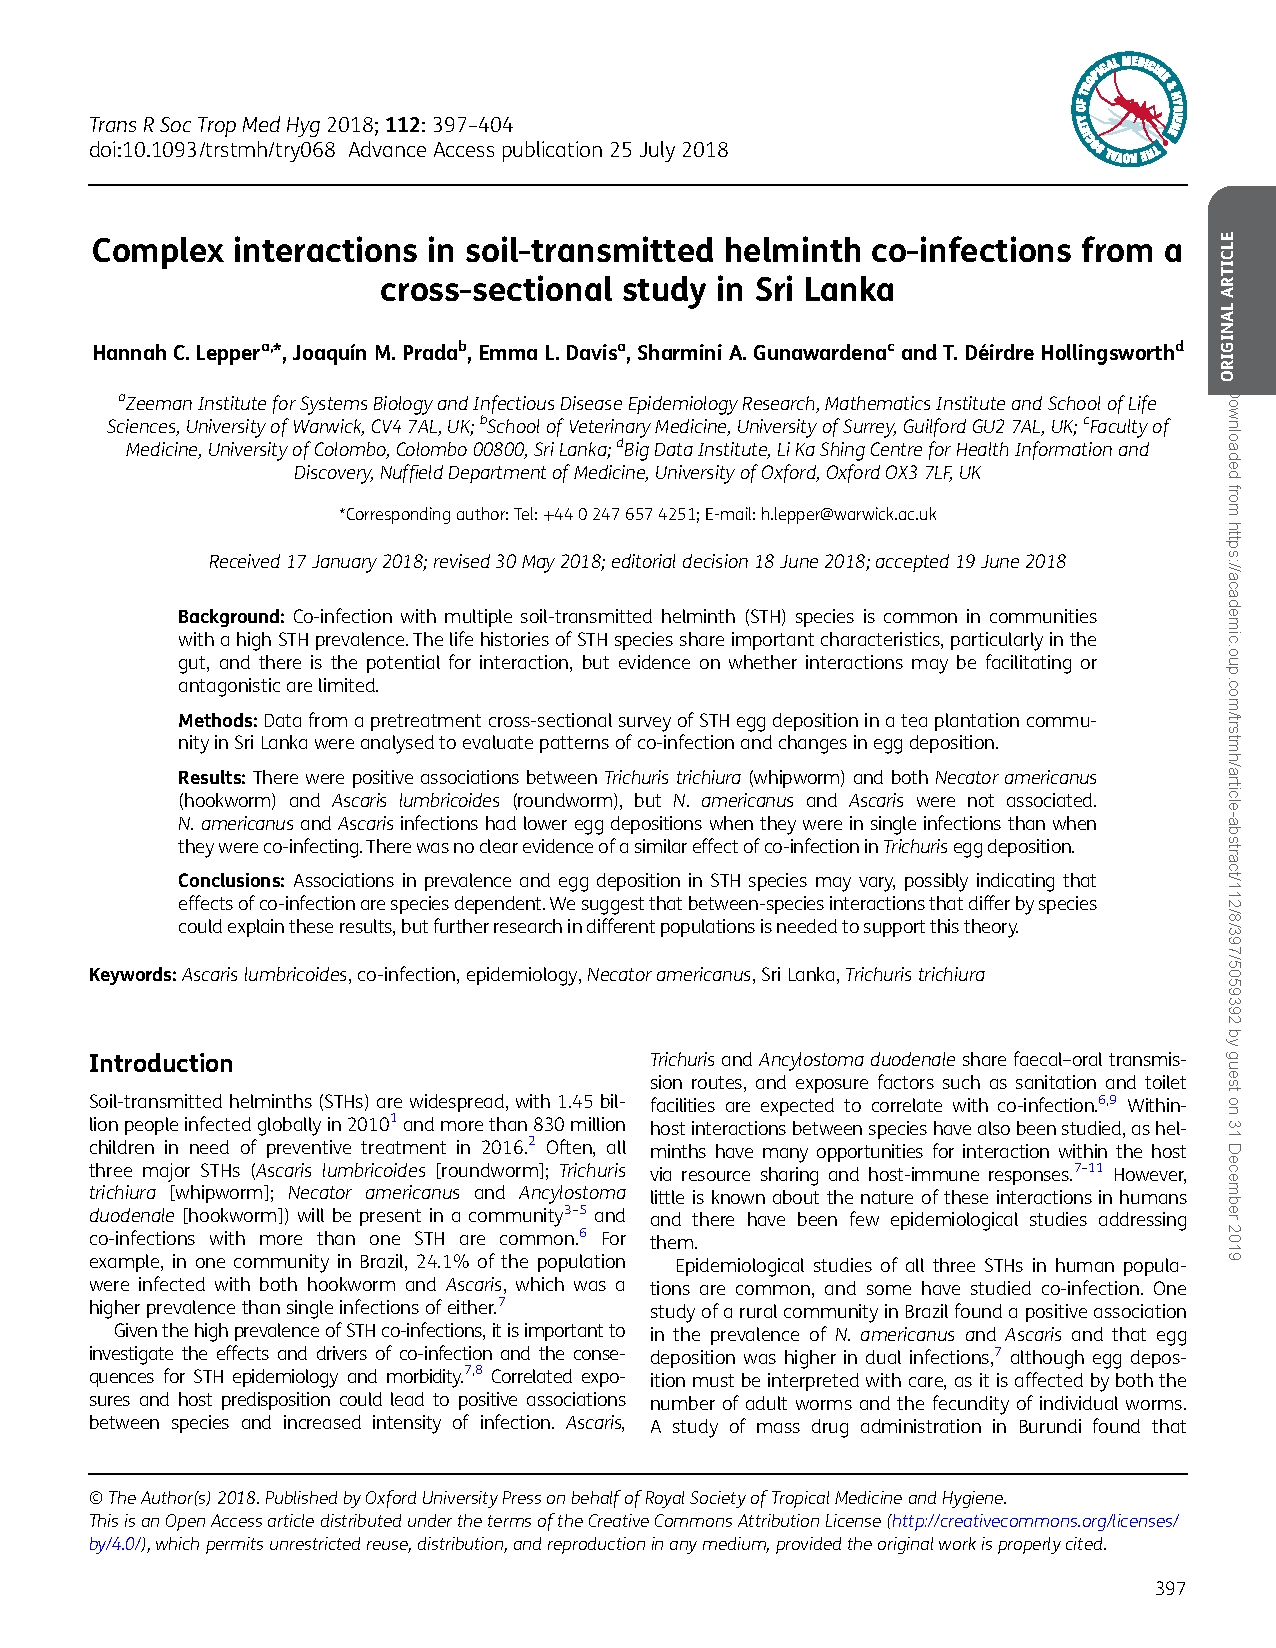
\includepdf[pages=-,pagecommand={},width=\textwidth+2cm,offset=20 -20]{LepperPaper.pdf}